\section{Spacings, irregularity and the cell distance}\label{ch:spacing}

On a window of finite height the errors of the P\'olya route, measured by the cell distance $d_{\rm cell}(\varepsilon)$ of Section~\ref{ch:distances}, are set by the spacings of the zeros, which follow the random matrix prediction already for the first $1700$ zeros.

\subsection{The cell distance to first order}\label{sec:ch15:first}

We use the cells $C_k=(b_{k-1},b_k]$ of Section~\ref{sec:ch7:cumulative}, with $\Theta=200$ and $K=N(\Theta)=79$, and the first order formula for $\mu_\varepsilon(C_k)-1$ derived there, whose remainder is $O(\varepsilon^3)$ (Remark~\ref{rem:ch7:cubic}); Exercise~\ref{ex:ch15:odd} gives its leading term. The formula needs only that the zeros below $\Theta$ be simple and on the line.

Under RH the formula becomes a sum over the ordinates. By Proposition~\ref{prop:struct}, $\rho_\varepsilon(\theta)=\sum_j[P_\varepsilon(\theta-\gamma_j)+P_\varepsilon(\theta+\gamma_j)]$ over all positive ordinates, and the kernel $P_\varepsilon(\cdot-\gamma)$ has distribution function $F_\varepsilon(y-\gamma)$, where $F_\varepsilon(y)=\frac12+\frac1\pi\arctan(y/\varepsilon)=\mathbf 1_{y\ge0}-\varepsilon/(\pi y)+O(\varepsilon^3/|y|^3)$ as $\varepsilon/|y|\to0$. No ordinate lies on a cell boundary, so
\[
\mu_\varepsilon(C_k)-1=-\frac\varepsilon\pi\sum_j\Big[\frac1{b_k-\gamma_j}-\frac1{b_{k-1}-\gamma_j}+\frac1{b_k+\gamma_j}-\frac1{b_{k-1}+\gamma_j}\Big]+O(\varepsilon^3),
\]
and by \eqref{eq:ch2:hadamard} with $s=i\theta$, $\Xi'/\Xi(\theta)=\sum_j[(\theta-\gamma_j)^{-1}+(\theta+\gamma_j)^{-1}]$ under RH, so the two expansions agree. Summing absolute values,
\[
\begin{aligned}
d_{\rm cell}(\varepsilon)&=\kappa_{\rm cell}\,\varepsilon+O(\varepsilon^3),\\
\kappa_{\rm cell}&=\frac1\pi\sum_k\Big|\sum_j\Big[\frac1{b_k-\gamma_j}-\frac1{b_{k-1}-\gamma_j}+\frac1{b_k+\gamma_j}-\frac1{b_{k-1}+\gamma_j}\Big]\Big| .
\end{aligned}
\]

Truncated to the first $1700$ ordinates, the zero sum gives $5.415$, against $\kappa_{\rm cell}=5.43665$ from the form in $\Xi'/\Xi$ and the observed slope $d_{\rm cell}(0.005)/0.005=5.43664$. The difference of $0.4$ per cent between $5.415$ and $5.43665$ is the contribution of the zeros above $\gamma_{1700}$. In the truncated formula the cell errors range from $-0.225\,\varepsilon$ to $+0.250\,\varepsilon$ (Figure~\ref{fig:ch15:cells}), with the two largest positive values at the end cells: at the last because $\Theta$ is not a midpoint between ordinates, and at the first because below $b_1$ there is only $\gamma_1$ and then the reflections $-\gamma_j$, which do not balance the zeros above $b_1$.

\begin{figure}[htbp]
\centering
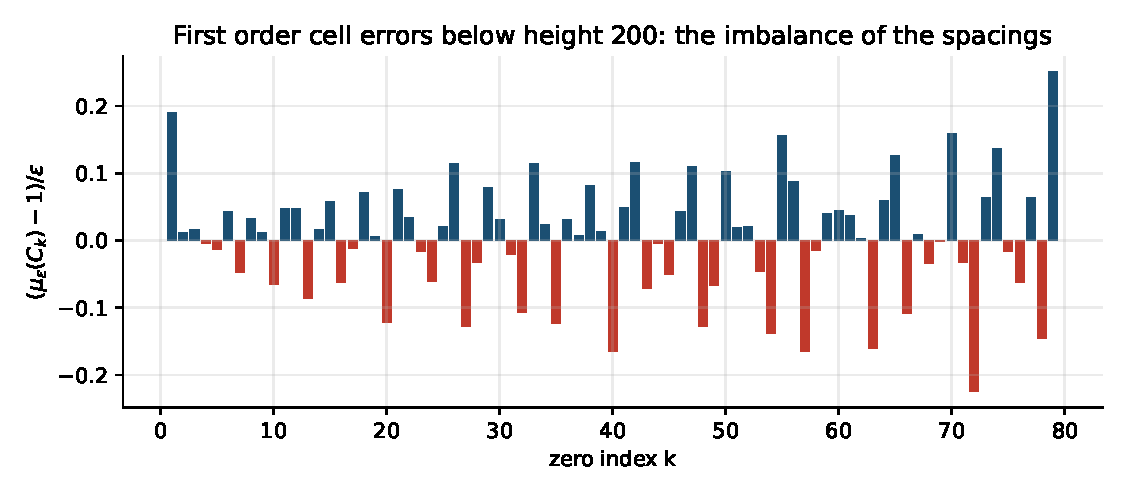
\includegraphics[width=0.85\textwidth]{fig/cells.pdf}
\caption{First order cell errors $(\mu_\varepsilon(C_k)-1)/\varepsilon$ for the $79$ cells below height $200$, computed from the first $1700$ ordinates.}
\label{fig:ch15:cells}
\end{figure}

The atoms $\theta=k\ge1$ of the sinh benchmark of Section~\ref{ch:ggc} and their reflections form the lattice $\mathbb Z$ without the point $0$. For the full lattice every cell $(k-\frac12,k+\frac12]$ would have mass exactly one, by periodicity, so the deficit of each cell is the mass that the missing kernel at $0$ would have put in it; the atom free interval $(0,\frac12]$, which the benchmark counts as a cell of mass zero, receives the mass $\frac12$ of the full lattice less that of the missing kernel:
\[
\mu_\varepsilon\big((k-\tfrac12,k+\tfrac12]\big)=1-\frac1\pi\arctan\frac{\varepsilon}{\varepsilon^2+k^2-\frac14},\qquad \mu_\varepsilon\big((0,\tfrac12]\big)=\frac1\pi\arctan(2\varepsilon).
\]
The interior cells therefore do not balance: each loses $\varepsilon/(\pi(k^2-\frac14))+O(\varepsilon^3)$, while $(0,\frac12]$ gains $2\varepsilon/\pi+O(\varepsilon^3)$. As $\sum_{k\le N}(k^2-\frac14)^{-1}=2-1/(N+\frac12)$, the cell distance of $N$ atoms is $(4-1/(N+\frac12))\,\varepsilon/\pi+O(\varepsilon^3)$, which is $1.26694\,\varepsilon$ for $N=50$, the constant $1.267$ of Section~\ref{ch:ggc}. With the convention used for the zeros, a first cell $(0,\frac32]$, it would be $(\frac43-1/(N+\frac12))/\pi=0.418$. For the zeros no cell is balanced, and the errors in Figure~\ref{fig:ch15:cells} do not decay along the window.

The constant vanishes exactly when the sum of $1/(b-x)$ over the ordinates and their reflections vanishes at every cell boundary $b$, as it does when these points are symmetric about every boundary. The lattice $\gamma_j=(j-\frac12)h$, whose reflections complete $(\mathbb Z+\frac12)h$, has every cell error zero, whereas the lattice of the benchmark does not. For the zeros every ordinate contributes to a cell error, with a weight that decays like $|C_k|/(\gamma_j-b_k)^2$. The two ordinates nearest an interior boundary are symmetric about it, so the asymmetry comes first from the next gaps on either side, and it is small when those gaps are equal.

\subsection{Spacings of the zeros and the Thorin density}\label{sec:ch15:spacings}

At height $\gamma$ the mean spacing of the zeros is $\Delta=2\pi/\log(\gamma/2\pi)$, as in Section~\ref{sec:ch13:visibility}. We unfold by $\tilde\gamma=\vartheta(\gamma)/\pi$. The $1699$ normalised spacings $\tilde\gamma_{k+1}-\tilde\gamma_k$ of the first $1700$ zeros, which lie below height $2198$, have variance $0.146$ and minimum $0.089$. Figure~\ref{fig:ch15:spacing} compares their histogram with the Wigner surmise for the Gaussian unitary ensemble, $p_{\rm W}(s)=\frac{32}{\pi^2}s^2e^{-4s^2/\pi}$, and with the Poisson law $e^{-s}$ of independent points. The histogram follows the surmise already at this height, including the quadratic repulsion at small spacings that Montgomery's pair correlation conjecture predicts \cite[pp.~183 and 184]{Montgomery73} and that Odlyzko observed at large height \cite{Odlyzko87}. The variance is below the surmise value $3\pi/8-1=0.178$; the spacing distribution approaches the unitary one only slowly with height \cite[p.~185]{Montgomery73}, \cite[Section 3]{BBLM06}.

\begin{figure}[htbp]
\centering
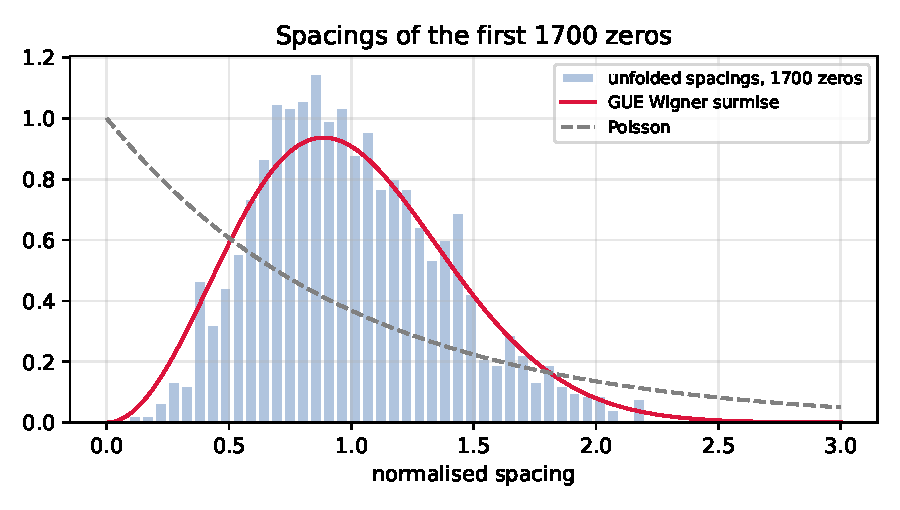
\includegraphics[width=0.72\textwidth]{fig/spacing.pdf}
\caption{The $1699$ unfolded spacings of the first $1700$ zeros against the GUE Wigner surmise and the Poisson law.}
\label{fig:ch15:spacing}
\end{figure}

Repulsion affects the Thorin density in two ways. First, it makes very small gaps rare but not absent. The smallest normalised spacing among the first $1700$ zeros, $0.089$, separates the ordinates $1977.17$ and $1977.27$, the pair that Section~\ref{ch:finite} moves off the line in Figure~\ref{fig:ch13:perturb}. By the Cauchy kernel criterion of Exercise~\ref{ex:ch5:cauchy}, an isolated pair of ordinates at distance $g$ in $\theta$ gives two peaks of $\rho_\varepsilon$ only for $\varepsilon<\sqrt3g/2$. The resolution needed to separate every pair on a window is therefore set by the smallest gap, and repulsion controls it: if the $N$ normalised spacings were independent, with density $p_{\rm W}(s)\propto s^2$ near zero, the smallest would be of order $N^{-1/3}$, which is $0.084$ for $N=1699$, close to the observed $0.089$.

Second, repulsion sets the scale of the local visibility condition of Section~\ref{sec:ch13:visibility}: to first order in $\varepsilon$, an off line zero at distance $d$ from the line makes $\rho_\varepsilon$ negative at its ordinate if and only if $2/d^2$ exceeds $\sum_j\delta_j^{-2}$, where $\delta_j$ are the distances from its ordinate to the other ordinates. The sum is dominated by the nearest neighbours, and repulsion makes it typically of order $\Delta^{-2}$, because $\E s^{-2}$ is finite for the surmise, where it equals $8/\pi$, and infinite for the Poisson law. With neighbours on a lattice of spacing $\Delta$, the density at the ordinate stays positive at small resolution once $d$ exceeds the threshold $(\sqrt6/\pi)\Delta\approx0.78\,\Delta$ of that section. Since $d<\frac12$, a zero hidden in this way can exist only where $\Delta<0.64$, that is above height about $1.1\times10^5$. Hidden here means hidden at the ordinate: beside it the density can be negative even when the condition predicts a positive value there (Exercise~\ref{ex:ch15:beside}).

The behaviour of the cell constant at large height is open (Section~\ref{ch:open}). In unfolded units the cell errors depend mainly on the nearby ordinates, so the sine kernel process of the unitary ensemble would predict their mean and fluctuations per cell; we have not computed that prediction. Computing the cell errors with Odlyzko's zeros near zero number $10^{12}$ \cite{Odlyzko87}, $10^{21}$ or $10^{22}$ \cite{Odlyzko01,OdlyzkoTables}, at heights about $2.7\times10^{11}$, $1.4\times10^{20}$ and $1.4\times10^{21}$, would compare the Thorin density with the spacing statistics of the zeros at large height. It needs the ordinates, which define the cells, and the hybrid evaluator of Section~\ref{sec:ch5:hybrid} for $\Xi'/\Xi$ at the cell boundaries. Section~\ref{ag:sec:margins} proposes the same comparison at large height for the positivity margins of the density, its values at the midpoints between consecutive ordinates.
